%%%%%%%%%%%%%%%%%%%%%%%%%%%%%%%%%%%%%%%%%
%  Kiqo User Guide 
%
% Important note:
% Chapter heading images should have a 2:1 width:height ratio,
% e.g. 920px width and 460px height.
%
%%%%%%%%%%%%%%%%%%%%%%%%%%%%%%%%%%%%%%%%%

%----------------------------------------------------------------------------------------
%	PACKAGES AND OTHER DOCUMENT CONFIGURATIONS
%----------------------------------------------------------------------------------------

\documentclass[11pt,fleqn]{book} % Default font size and left-justified equations

\usepackage[top=3cm,bottom=3cm,left=3.2cm,right=3.2cm,headsep=10pt,letterpaper]{geometry} % Page margins

\usepackage{xcolor} % Required for specifying colors by name
\definecolor{ocre}{RGB}{52,177,201} % Define the orange color used for highlighting throughout the book

\usepackage{float}
\usepackage{booktabs}

% Font Settings
\usepackage{avant} % Use the Avantgarde font for headings
%\usepackage{times} % Use the Times font for headings
\usepackage{mathptmx} % Use the Adobe Times Roman as the default text font together with math symbols from the Sym­bol, Chancery and Com­puter Modern fonts

\usepackage{microtype} % Slightly tweak font spacing for aesthetics
\usepackage[utf8]{inputenc} % Required for including letters with accents
\usepackage[T1]{fontenc} % Use 8-bit encoding that has 256 glyphs

\usepackage{menukeys}

% Bibliography
%\usepackage[style=alphabetic,sorting=nyt,sortcites=true,autopunct=true,babel=hyphen,hyperref=true,abbreviate=false,backref=true,backend=biber]{biblatex}
%\addbibresource{bibliography.bib} % BibTeX bibliography file
%\defbibheading{bibempty}{}

%----------------------------------------------------------------------------------------
%	VARIOUS REQUIRED PACKAGES
%----------------------------------------------------------------------------------------

\usepackage{titlesec} % Allows customization of titles

\usepackage{graphicx} % Required for including pictures
\graphicspath{{Pictures/}} % Specifies the directory where pictures are stored

\usepackage{lipsum} % Inserts dummy text

\usepackage{tikz} % Required for drawing custom shapes

\usepackage[english]{babel} % English language/hyphenation

\usepackage{enumitem} % Customize lists
\setlist{nolistsep} % Reduce spacing between bullet points and numbered lists

\usepackage{booktabs} % Required for nicer horizontal rules in tables

\usepackage{eso-pic} % Required for specifying an image background in the title page

%----------------------------------------------------------------------------------------
%	MAIN TABLE OF CONTENTS
%----------------------------------------------------------------------------------------

\usepackage{titletoc} % Required for manipulating the table of contents

\contentsmargin{0cm} % Removes the default margin
% Chapter text styling
\titlecontents{chapter}[1.25cm] % Indentation
{\addvspace{15pt}\large\sffamily\bfseries} % Spacing and font options for chapters
{\color{ocre!60}\contentslabel[\Large\thecontentslabel]{1.25cm}\color{ocre}} % Chapter number
{}  
{\color{ocre!60}\normalsize\sffamily\bfseries\;\titlerule*[.5pc]{.}\;\thecontentspage} % Page number
% Section text styling
\titlecontents{section}[1.25cm] % Indentation
{\addvspace{5pt}\sffamily\bfseries} % Spacing and font options for sections
{\contentslabel[\thecontentslabel]{1.25cm}} % Section number
{}
{\sffamily\hfill\color{black}\thecontentspage} % Page number
[]
% Subsection text styling
\titlecontents{subsection}[1.25cm] % Indentation
{\addvspace{1pt}\sffamily\small} % Spacing and font options for subsections
{\contentslabel[\thecontentslabel]{1.25cm}} % Subsection number
{}
{\sffamily\;\titlerule*[.5pc]{.}\;\thecontentspage} % Page number
[] 

%----------------------------------------------------------------------------------------
%	MINI TABLE OF CONTENTS IN CHAPTER HEADS
%----------------------------------------------------------------------------------------

% Section text styling
\titlecontents{lsection}[0em] % Indendating
{\footnotesize\sffamily} % Font settings
{}
{}
{}

% Subsection text styling
\titlecontents{lsubsection}[.5em] % Indentation
{\normalfont\footnotesize\sffamily} % Font settings
{}
{}
{}
 
%----------------------------------------------------------------------------------------
%	PAGE HEADERS
%----------------------------------------------------------------------------------------

\usepackage{fancyhdr} % Required for header and footer configuration

\pagestyle{fancy}
\renewcommand{\chaptermark}[1]{\markboth{\sffamily\normalsize\bfseries\chaptername\ \thechapter.\ #1}{}} % Chapter text font settings
\renewcommand{\sectionmark}[1]{\markright{\sffamily\normalsize\thesection\hspace{5pt}#1}{}} % Section text font settings
\fancyhf{} \fancyhead[LE,RO]{\sffamily\normalsize\thepage} % Font setting for the page number in the header
\fancyhead[LO]{\rightmark} % Print the nearest section name on the left side of odd pages
\fancyhead[RE]{\leftmark} % Print the current chapter name on the right side of even pages
\renewcommand{\headrulewidth}{0.5pt} % Width of the rule under the header
\addtolength{\headheight}{2.5pt} % Increase the spacing around the header slightly
\renewcommand{\footrulewidth}{0pt} % Removes the rule in the footer
\fancypagestyle{plain}{\fancyhead{}\renewcommand{\headrulewidth}{0pt}} % Style for when a plain pagestyle is specified

% Removes the header from odd empty pages at the end of chapters
\makeatletter
\renewcommand{\cleardoublepage}{
\clearpage\ifodd\c@page\else
\hbox{}
\vspace*{\fill}
\thispagestyle{empty}
\clearpage
\fi}

%----------------------------------------------------------------------------------------
%	THEOREM STYLES
%----------------------------------------------------------------------------------------

\usepackage{amsmath,amsfonts,amssymb,amsthm} % For math equations, theorems, symbols, etc

\newcommand{\intoo}[2]{\mathopen{]}#1\,;#2\mathclose{[}}
\newcommand{\ud}{\mathop{\mathrm{{}d}}\mathopen{}}
\newcommand{\intff}[2]{\mathopen{[}#1\,;#2\mathclose{]}}
\newtheorem{notation}{Notation}[chapter]

%%%%%%%%%%%%%%%%%%%%%%%%%%%%%%%%%%%%%%%%%%%%%%%%%%%%%%%%%%%%%%%%%%%%%%%%%%%
%%%%%%%%%%%%%%%%%%%% dedicated to boxed/framed environements %%%%%%%%%%%%%%
%%%%%%%%%%%%%%%%%%%%%%%%%%%%%%%%%%%%%%%%%%%%%%%%%%%%%%%%%%%%%%%%%%%%%%%%%%%
\newtheoremstyle{ocrenumbox}% % Theorem style name
{0pt}% Space above
{0pt}% Space below
{\normalfont}% % Body font
{}% Indent amount
{\small\bf\sffamily\color{ocre}}% % Theorem head font
{\;}% Punctuation after theorem head
{0.25em}% Space after theorem head
{\small\sffamily\color{ocre}\thmname{#1}\nobreakspace\thmnumber{\@ifnotempty{#1}{}\@upn{#2}}% Theorem text (e.g. Theorem 2.1)
\thmnote{\nobreakspace\the\thm@notefont\sffamily\bfseries\color{black}---\nobreakspace#3.}} % Optional theorem note
\renewcommand{\qedsymbol}{$\blacksquare$}% Optional qed square

\newtheoremstyle{blacknumex}% Theorem style name
{5pt}% Space above
{5pt}% Space below
{\normalfont}% Body font
{} % Indent amount
{\small\bf\sffamily}% Theorem head font
{\;}% Punctuation after theorem head
{0.25em}% Space after theorem head
{\small\sffamily{\tiny\ensuremath{\blacksquare}}\nobreakspace\thmname{#1}\nobreakspace\thmnumber{\@ifnotempty{#1}{}\@upn{#2}}% Theorem text (e.g. Theorem 2.1)
\thmnote{\nobreakspace\the\thm@notefont\sffamily\bfseries---\nobreakspace#3.}}% Optional theorem note

\newtheoremstyle{blacknumbox} % Theorem style name
{0pt}% Space above
{0pt}% Space below
{\normalfont}% Body font
{}% Indent amount
{\small\bf\sffamily}% Theorem head font
{\;}% Punctuation after theorem head
{0.25em}% Space after theorem head
{\small\sffamily\thmname{#1}\nobreakspace\thmnumber{\@ifnotempty{#1}{}\@upn{#2}}% Theorem text (e.g. Theorem 2.1)
\thmnote{\nobreakspace\the\thm@notefont\sffamily\bfseries---\nobreakspace#3.}}% Optional theorem note

%%%%%%%%%%%%%%%%%%%%%%%%%%%%%%%%%%%%%%%%%%%%%%%%%%%%%%%%%%%%%%%%%%%%%%%%%%%
%%%%%%%%%%%%% dedicated to non-boxed/non-framed environements %%%%%%%%%%%%%
%%%%%%%%%%%%%%%%%%%%%%%%%%%%%%%%%%%%%%%%%%%%%%%%%%%%%%%%%%%%%%%%%%%%%%%%%%%
\newtheoremstyle{ocrenum}% % Theorem style name
{5pt}% Space above
{5pt}% Space below
{\normalfont}% % Body font
{}% Indent amount
{\small\bf\sffamily\color{ocre}}% % Theorem head font
{\;}% Punctuation after theorem head
{0.25em}% Space after theorem head
{\small\sffamily\color{ocre}\thmname{#1}\nobreakspace\thmnumber{\@ifnotempty{#1}{}\@upn{#2}}% Theorem text (e.g. Theorem 2.1)
\thmnote{\nobreakspace\the\thm@notefont\sffamily\bfseries\color{black}---\nobreakspace#3.}} % Optional theorem note
\renewcommand{\qedsymbol}{$\blacksquare$}% Optional qed square
\makeatother

% Defines the theorem text style for each type of theorem to one of the three styles above
\newcounter{dummy} 
\numberwithin{dummy}{section}
\theoremstyle{ocrenumbox}
\newtheorem{theoremeT}[dummy]{Theorem}
\newtheorem{problem}{Problem}[chapter]
\newtheorem{exerciseT}{Exercise}[chapter]
\theoremstyle{blacknumex}
\newtheorem{exampleT}{Example}[chapter]
\theoremstyle{blacknumbox}
\newtheorem{vocabulary}{Vocabulary}[chapter]
\newtheorem{definitionT}{Definition}[section]
\newtheorem{corollaryT}[dummy]{Corollary}
\theoremstyle{ocrenum}
\newtheorem{proposition}[dummy]{Proposition}

%----------------------------------------------------------------------------------------
%	DEFINITION OF COLORED BOXES
%----------------------------------------------------------------------------------------

\RequirePackage[framemethod=default]{mdframed} % Required for creating the theorem, definition, exercise and corollary boxes

% Theorem box
\newmdenv[skipabove=7pt,
skipbelow=7pt,
backgroundcolor=black!5,
linecolor=ocre,
innerleftmargin=5pt,
innerrightmargin=5pt,
innertopmargin=5pt,
leftmargin=0cm,
rightmargin=0cm,
innerbottommargin=5pt]{tBox}

% Exercise box	  
\newmdenv[skipabove=7pt,
skipbelow=7pt,
rightline=false,
leftline=true,
topline=false,
bottomline=false,
backgroundcolor=ocre!10,
linecolor=ocre,
innerleftmargin=5pt,
innerrightmargin=5pt,
innertopmargin=5pt,
innerbottommargin=5pt,
leftmargin=0cm,
rightmargin=0cm,
linewidth=4pt]{eBox}	

% Definition box
\newmdenv[skipabove=7pt,
skipbelow=7pt,
rightline=false,
leftline=true,
topline=false,
bottomline=false,
linecolor=ocre,
innerleftmargin=5pt,
innerrightmargin=5pt,
innertopmargin=0pt,
leftmargin=0cm,
rightmargin=0cm,
linewidth=4pt,
innerbottommargin=0pt]{dBox}	

% Corollary box
\newmdenv[skipabove=7pt,
skipbelow=7pt,
rightline=false,
leftline=true,
topline=false,
bottomline=false,
linecolor=gray,
backgroundcolor=black!5,
innerleftmargin=5pt,
innerrightmargin=5pt,
innertopmargin=5pt,
leftmargin=0cm,
rightmargin=0cm,
linewidth=4pt,
innerbottommargin=5pt]{cBox}

% Creates an environment for each type of theorem and assigns it a theorem text style from the "Theorem Styles" section above and a colored box from above
\newenvironment{theorem}{\begin{tBox}\begin{theoremeT}}{\end{theoremeT}\end{tBox}}
\newenvironment{exercise}{\begin{eBox}\begin{exerciseT}}{\hfill{\color{ocre}\tiny\ensuremath{\blacksquare}}\end{exerciseT}\end{eBox}}				  
\newenvironment{definition}{\begin{dBox}\begin{definitionT}}{\end{definitionT}\end{dBox}}	
\newenvironment{example}{\begin{exampleT}}{\hfill{\tiny\ensuremath{\blacksquare}}\end{exampleT}}		
\newenvironment{corollary}{\begin{cBox}\begin{corollaryT}}{\end{corollaryT}\end{cBox}}	

%----------------------------------------------------------------------------------------
%	REMARK ENVIRONMENT
%----------------------------------------------------------------------------------------

\newenvironment{remark}{\par\vspace{10pt}\small % Vertical white space above the remark and smaller font size
\begin{list}{}{
\leftmargin=35pt % Indentation on the left
\rightmargin=25pt}\item\ignorespaces % Indentation on the right
\makebox[-2.5pt]{\begin{tikzpicture}[overlay]
\node[draw=ocre!60,line width=1pt,circle,fill=ocre!25,font=\sffamily\bfseries,inner sep=2pt,outer sep=0pt] at (-15pt,0pt){\textcolor{ocre}{R}};\end{tikzpicture}} % Orange R in a circle
\advance\baselineskip -1pt}{\end{list}\vskip5pt} % Tighter line spacing and white space after remark

%----------------------------------------------------------------------------------------
%	SECTION NUMBERING IN THE MARGIN
%----------------------------------------------------------------------------------------

\makeatletter
\renewcommand{\@seccntformat}[1]{\llap{\textcolor{ocre}{\csname the#1\endcsname}\hspace{1em}}}                    
\renewcommand{\section}{\@startsection{section}{1}{\z@}
{-4ex \@plus -1ex \@minus -.4ex}
{1ex \@plus.2ex }
{\normalfont\large\sffamily\bfseries}}
\renewcommand{\subsection}{\@startsection {subsection}{2}{\z@}
{-3ex \@plus -0.1ex \@minus -.4ex}
{0.5ex \@plus.2ex }
{\normalfont\sffamily\bfseries}}
\renewcommand{\subsubsection}{\@startsection {subsubsection}{3}{\z@}
{-2ex \@plus -0.1ex \@minus -.2ex}
{.2ex \@plus.2ex }
{\normalfont\small\sffamily\bfseries}}                        
\renewcommand\paragraph{\@startsection{paragraph}{4}{\z@}
{-2ex \@plus-.2ex \@minus .2ex}
{.1ex}
{\normalfont\small\sffamily\bfseries}}

%----------------------------------------------------------------------------------------
%	HYPERLINKS IN THE DOCUMENTS
%----------------------------------------------------------------------------------------

% For an unclear reason, the package should be loaded now and not later
\usepackage{hyperref}
\hypersetup{hidelinks,backref=true,pagebackref=true,hyperindex=true,colorlinks=false,breaklinks=true,urlcolor= ocre,bookmarks=true,bookmarksopen=false,pdftitle={Title},pdfauthor={Author}}

%----------------------------------------------------------------------------------------
%	CHAPTER HEADINGS
%----------------------------------------------------------------------------------------

% The set-up below should be (sadly) manually adapted to the overall margin page septup controlled by the geometry package loaded in the main.tex document. It is possible to implement below the dimensions used in the goemetry package (top,bottom,left,right)... TO BE DONE

\newcommand{\thechapterimage}{}
\newcommand{\chapterimage}[1]{\renewcommand{\thechapterimage}{#1}}

% Numbered chapters with mini tableofcontents
\def\thechapter{\arabic{chapter}}
\def\@makechapterhead#1{
\thispagestyle{empty}
{\centering \normalfont\sffamily
\ifnum \c@secnumdepth >\m@ne
\if@mainmatter
\startcontents
\begin{tikzpicture}[remember picture,overlay]
\node at (current page.north west)
{\begin{tikzpicture}[remember picture,overlay]
\node[anchor=north west,inner sep=0pt] at (0,0) {\includegraphics[width=\paperwidth]{\thechapterimage}};
%%%%%%%%%%%%%%%%%%%%%%%%%%%%%%%%%%%%%%%%%%%%%%%%%%%%%%%%%%%%%%%%%%%%%%%%%%%%%%%%%%%%%
% Commenting the 3 lines below removes the small contents box in the chapter heading
%\fill[color=ocre!10!white,opacity=.6] (1cm,0) rectangle (8cm,-7cm);
%\node[anchor=north west] at (1.1cm,.35cm) {\parbox[t][8cm][t]{6.5cm}{\huge\bfseries\flushleft \printcontents{l}{1}{\setcounter{tocdepth}{2}}}};
\draw[anchor=west] (5cm,-9cm) node [rounded corners=20pt,fill=ocre!10!white,text opacity=1,draw=ocre,draw opacity=1,line width=1.5pt,fill opacity=.6,inner sep=12pt]{\huge\sffamily\bfseries\textcolor{black}{\thechapter. #1\strut\makebox[22cm]{}}};
%%%%%%%%%%%%%%%%%%%%%%%%%%%%%%%%%%%%%%%%%%%%%%%%%%%%%%%%%%%%%%%%%%%%%%%%%%%%%%%%%%%%%
\end{tikzpicture}};
\end{tikzpicture}}
\par\vspace*{230\p@}
\fi
\fi}

% Unnumbered chapters without mini tableofcontents (could be added though) 
\def\@makeschapterhead#1{
\thispagestyle{empty}
{\centering \normalfont\sffamily
\ifnum \c@secnumdepth >\m@ne
\if@mainmatter
\begin{tikzpicture}[remember picture,overlay]
\node at (current page.north west)
{\begin{tikzpicture}[remember picture,overlay]
\node[anchor=north west,inner sep=0pt] at (0,0) {\includegraphics[width=\paperwidth]{\thechapterimage}};
\draw[anchor=west] (5cm,-9cm) node [rounded corners=20pt,fill=ocre!10!white,fill opacity=.6,inner sep=12pt,text opacity=1,draw=ocre,draw opacity=1,line width=1.5pt]{\huge\sffamily\bfseries\textcolor{black}{#1\strut\makebox[22cm]{}}};
\end{tikzpicture}};
\end{tikzpicture}}
\par
\clearpage
\vspace*{230\p@}
\fi
\fi
}
\makeatother % Insert the commands.tex file which contains the majority of the structure behind the template

\begin{document}

%----------------------------------------------------------------------------------------
%	TITLE PAGE
%----------------------------------------------------------------------------------------

\begingroup
\thispagestyle{empty}
\center{
\includegraphics[scale=0.25]{badgecolour}} % Thirsty Goat Badge 
%\AddToShipoutPicture*{\put(0,0){\includegraphics[scale=1.25]{esahubble}}} % Image background
\centering
\vspace*{5cm}
\par\normalfont\fontsize{35}{35}\sffamily\selectfont
\textbf{Kiqo}
{\LARGE A less horrible Agilefant}\par % Book title
\vspace*{1cm}
{\Huge User Guide}\par % Author name
\endgroup

%----------------------------------------------------------------------------------------
%	TABLE OF CONTENTS
%----------------------------------------------------------------------------------------

\tableofcontents % Print the table of contents itself

%----------------------------------------------------------------------------------------
%	CHAPTER 1
%----------------------------------------------------------------------------------------
\chapter{Introduction}

\section{Kiqo}
Kiqo is an agile project management tool. Like its namesake, New Zealand's most hardy breed of goat, Kiqo is sweet as.

\section{Quick Start}
\begin{itemize}
    \item All items can be created using \menu{File > New >} or by using the keyboard shortcuts which can be found
    in the appendix.
    \item All items can be edited using \keys{\ctrl + E}\footnote{On Mac, use the command key \keys{\cmd} in place of \keys{\ctrl}.}
     or by right clicking on the item and selecting edit.
    \item All items can be deleted using \keys{\ctrl + D} or by right clicking on the item and selecting delete.
    \item To save use either \menu{File > Save} or \keys{\ctrl + S}.
    \item To load an existing .json file use either \menu{File > Load} or \keys{\ctrl + O} and select the file using the file chooser.
    \item Undo an action using either \menu{Edit > Undo} or \keys{\ctrl + Z}.
    \item Redo an action using either \menu{Edit > Redo} or \keys{\ctrl + \shift + Z}.
    \item To revert to the last save point use \menu{File > Revert}.
\end{itemize}
\clearpage

\section{Window Layout}
The main Kiqo workspace is shown in Figure~\ref{fig:mainwindow}.

\begin{figure}[H]
  \centering
  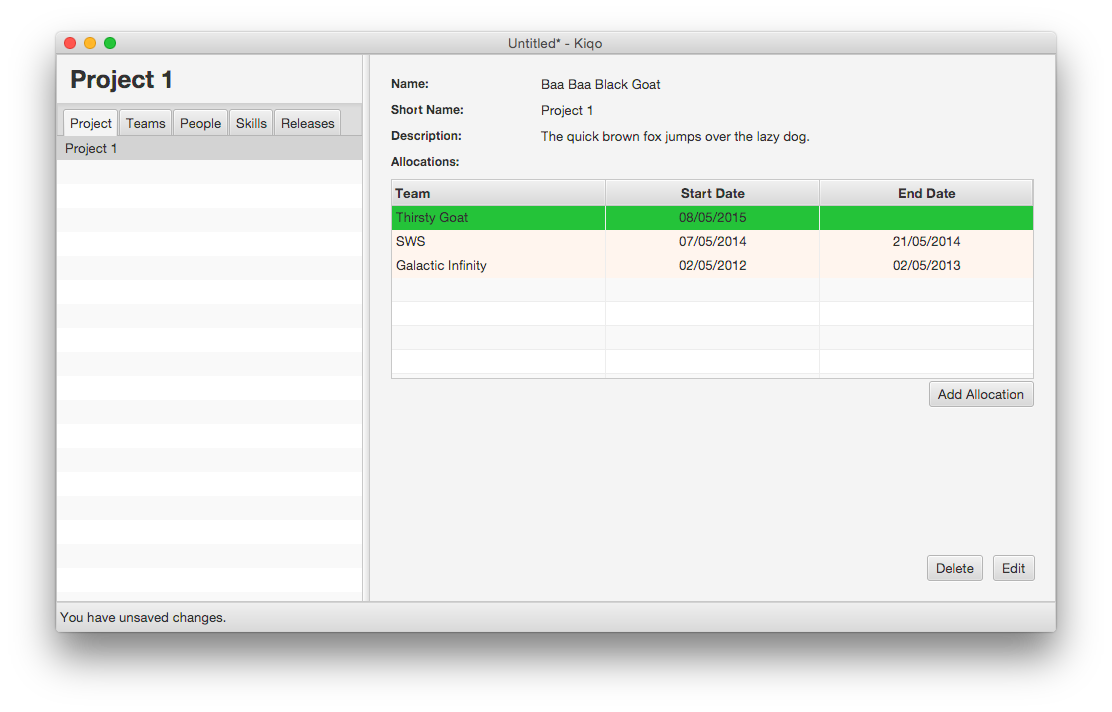
\includegraphics[scale=0.32]{mainwindow}
  \caption{The main Kiqo window.\label{fig:mainwindow}}
\end{figure}

\begin{enumerate}
\item Menu bar / Window title - The window title shows the organisation name. An asterisk next to the organisation name indicates that there are unsaved changes.
The menu bar contains commands for creating items, saving and loading files, generating reports and more.
\item Side bar - The sidebar gives an overview of the items in the organisaiton and allows you to select them.
There are three ways of changing the view to show relevant information.
    \begin{itemize}
      \item From the menu bar, use \menu{View > } and select the item.
      \item From clicking the selection tabs shown in Figure~\ref{fig:mainwindow}
      \item By using the keyboard shortcuts \keys{\ctrl + 1-4}
    \end{itemize}
    The items shown in the sidebar are automatically sorted in alphabetical order.
\item Details viewer - The details viewer displays the details of the item selected in the side bar.
\item Status bar - The status bar indicates if there are any unsaved changes.
\end{enumerate}


%----------------------------------------------------------------------------------------
%	CHAPTER 2
%----------------------------------------------------------------------------------------
\chapter{Items}
\section{Organisation}
An organisation is the root element of the hierarchy. An organisation contains projects, teams, people, skills, backlogs and stories.
A new organisation is automatically loaded when Kiqo is initially opened. An existing organisation can also be loaded
from a .json file. To create a new organisation use \menu{File > New > Organisation}. An organisation can be saved using
either \menu{File > Save} or \keys{ctrl + S}.

\section{Projects \& Releases}
\subsection{Create a project}
    \begin{itemize}
        \item From the menu bar, use \menu{File > New... > Project}.
        \item Use the keyboard shortcut \keys{\ctrl + N}.
    \end{itemize}
    You will then be prompted to enter the details of the new project.

    \begin{figure}[h]
        \centering
        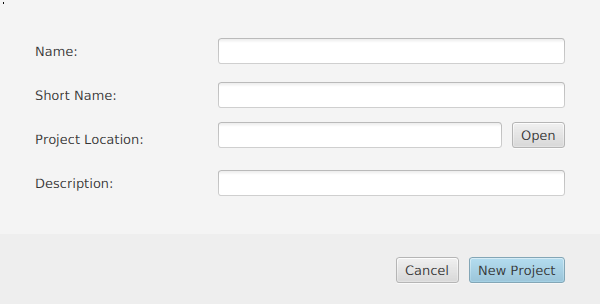
\includegraphics[scale=0.32]{newproject}
        \caption{The new project window.\label{newproject}}
    \end{figure}

\subsection{Create a Release}
    \begin{itemize}
        \item To create a release use \menu{File > New... > Release}.
        \item Use the keyboard shortcut \keys{\ctrl + R}.
    \end{itemize}
    The release will be added to the project selected in the creation dialog.
    The releases for a project can be found under the projects releases heading in the tree view.

\section{People \& Skills}
\subsection{People}
A person can be created, saved and edited in the same way as a project.
\subsection{Skills}
There are two important skills which cannot be modified: 
\begin{itemize}
  \item The Product Owner (PO) skill
  \item The Scrum Master (SM) skill
\end{itemize}
New skills can be created, edited and deleted.
\begin{itemize}
  \item Adding a new skill to the Project displays the skill in the Skills list view. If a skill exists, by default the
  first skill is shown in the details pane, unless another skill in the list is selected.
  \item Go to the skills selection pane in edit or create person and click the > arrow to add one skill to a person
  or >> to add all existing skills.
  \item In the skills selection pane click the < arrow to remove one skill or << to remove all assigned skills.
\end{itemize}

\begin{figure}[H]
  \centering
  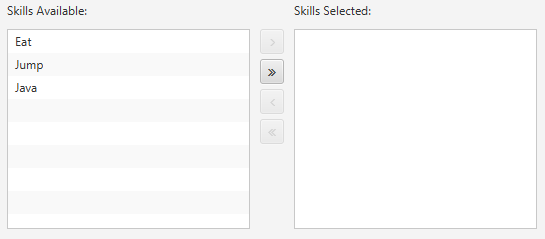
\includegraphics[scale=0.32]{skillsSelectionPane}
  \caption{The skills selection pane.\label{skillsSelectionPane}}
\end{figure}

\section{Teams, Roles \& Allocations}
\subsection{Team Maintenance (including Roles)}
\begin{itemize}
  \item Adding a new team to the Project displays the team in the Teams list view.
  \item The members of the selected team are displayed in the team details pane.
  \item In edit or create team, use the person selection pane and click the > arrow to add one person to a team
  or >> to add all available people.
  \item In the person selection pane, click the < arrow to remove one person or << to remove all assigned people.
  \item Use the radio buttons to nominate a Product Owner, Scrum Master and/or Development Team members. Only team members who
   possess the relevant skill may be nominated.
\end{itemize}

\subsection{Project Allocation}
\begin{itemize}
  \item Teams can be allocated to projects. A team can only be allocated to one project at a time.
  \item In the project tab a team can be allocated to a project by clicking the 'Allocate Teams'.
  \item Select a team from the from the dropdown list in create Allocation dialog and choose a start and an end date.
  \item Edit an allocation by clicking on a row and then changing the start or end date with the date picker.
  \item Delete an allocation by right clicking on its row and selecting 'Delete Allocation'.
\end{itemize}
\section{Backlogs \& Stories}

\subsection{Backlogs}

\begin{itemize}
\item Backlogs can be created when there is an existing project and at least one person with the product owner skill.
\item The owner of a backlog must have the product owner skill. 
\item Stories can be added to a backlog.
\end{itemize}

\subsubsection{Highlight Story State}
A backlog can show the current states of the stories it contains by toggling the check button located bellow the story table inside the backlog details pane.
If highlighting has been enabled a colour chip will be displayed on each row of the story table.
\begin{itemize}
\item A red chip indiciates that the story has a lower priority than a story that depends on it.
\item A orange chip indicates that the story is ready to be estimated.
\item A green chip indicates that the story is ready.
\end{itemize}


\subsection{Stories}

\begin{itemize}
  \item Stories can be added to a project and assigned a priority.
  \item The priority must be an integer between 1000 and -1000, inclusive.
\end{itemize}

\subsubsection{Estimation}
Stories can be estimated according to any one of these scales:
\begin{itemize}
\item Pseudo-Fibonnaci \textit{Default}
\item T-Shirt Sizes
\item Dog Breeds
\end{itemize}
The estimation scale is the same for all stories in a backlog.
share its backlog. Stories within a backlog that use a different estimation
scale will have their scale changed to that of the backlog, and the estimation unset.

\subsubsection{Acceptance Criteria}
Acceptance criteria can be added to a story and be assigned a state of readiness to help the user determine whether the
story is ready to begin. The readiness can be one of three states (ready/not ready/undetermined).
\begin{itemize}
  \item To create an acceptance criteria, inside the story detail pane, press the \menu{+} button under the acceptance critera table
  view.
  \item To change the readiness state of the acceptance critera, a toggle button on the right hand side of the tableview
  can be pressed repeatedly to alter the state.
  \item To rearrange the list of acceptance critera, click (and hold) within an acceptance critera cell (located within the tableview)
  and drag the cell up or down inside the tableview. Once the click has been released the acceptance critera will be
  dropped at that location and the order of the acceptance critera changed.
\end{itemize}

\subsubsection{Readiness}
A story can be marked as ready when the following criteria are met:
\begin{itemize}
\item the story belongs to a Backlog
\item the story is estimated
\item the story has at least one Acceptance Criterion
\end{itemize}

\subsubsection{Dependencies}
Some stories may depend on the completion of others. This information can be
added in the story form. 
Not all stories are available to be added as dependencies. Eligible stories must
meet the following criteria:
\begin{itemize}
\item the story is in the same backlog
\item adding the story as a dependency will not create a cyclic dependency
(cyclic dependencies are chains of dependencies that end with the story where
they begin)
\end{itemize}


%----------------------------------------------------------------------------------------
%	CHAPTER 3
%----------------------------------------------------------------------------------------
\chapter{Other Features}
\section{Report Generation}
The report generator gives the user the ability to generate reports in yaml format (http://yaml.org).
\begin{itemize}
  \item \menu{File > Generate > Status Report} Opens a dialog prompting you for the type of items to be in the report
  e.g. Projects, Teams, People etc. You can then select which of these items will be in the report e.g. Team 1 and
  Team 3.
  \item Clicking \keys{Generate Report} Prompts you for a valid save location on the local disk drive.
  \item Clicking \keys{Save} will generate the report and save it to the location set previously.
\end{itemize}

\begin{figure}[H]
  \centering
  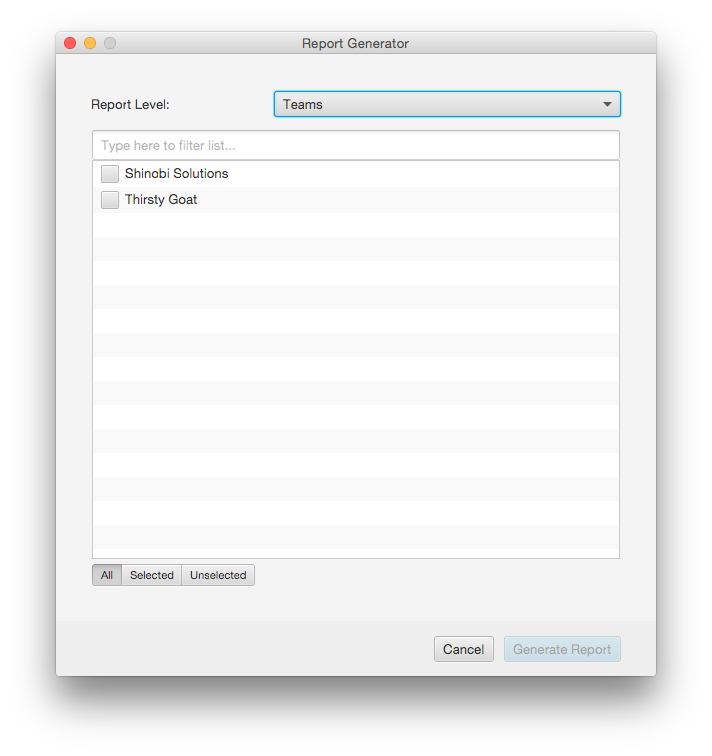
\includegraphics[scale=0.32]{reportForm}
  \caption{Report Generation Form.\label{reportForm}}
\end{figure}

\section{Undo, Redo, Revert}
\paragraph{}
Selecting \menu{Edit > Undo} will undo the last operation made to the organisation. It is important to note that any
new changes made after \textit{undoing} changes, will empty the
\textit{redo-able} operations. Be sure to save your organisation often to avoid
unrecoverable changes.

\paragraph{}
\menu{Edit > Redo} will redo the last operation that has been \textit{undone}.

\paragraph{}
Selecting \menu{File > Revert} will prompt the user that any unsaved changes will be lost, before reverting
to the previously saved state. If the organisation has not previously been saved, then it will be reverted
to a blank organisation. Note that the \textit{undo-able} operations will be preserved for the particular save state.

\section{Search}
Search gives the user the ability to find items that match a search query.

\paragraph{}
Selecting \menu{File > Search} will display the search toolbar. Whenever a character is entered into the search box the
results that match will be displayed bellow the text area.

\paragraph{}
If the seach result inside the list is clicked it will take the user to the location of that object.


%----------------------------------------------------------------------------------------
%	CHAPTER 4
%----------------------------------------------------------------------------------------
\appendix
\chapter{Appendix}
\clearpage

\section{Keyboard Shortcuts}

\textbf{Note:} On Mac the command key \keys{\cmd} should be used
  in place of \keys{\ctrl}.

\begin{table}[h]
  \renewcommand{\arraystretch}{1.5} % Increase space between rows
  \centering
  \begin{tabular}{lc}
    \toprule
    Action & Shortcut \\
    \midrule
    Create New Project & \keys{\ctrl + N} \\
    Create New Release & \keys{\ctrl + R} \\
    Create New Team & \keys{\ctrl + T} \\
    Create New Person & \keys{\ctrl + P} \\
    Create New Skill & \keys{\ctrl + K} \\
    Create New Story & \keys{\ctrl + Y} \\
    Open Organisation & \keys{\ctrl + O} \\
    Save Organisation & \keys{\ctrl + S} \\
    Save Organisation As & \keys{\ctrl + \shift + S} \\
    Undo & \keys{\ctrl + Z} \\
    Redo & \keys{\ctrl + \shift + Z} \\
    Edit Selected Item & \keys{\ctrl + E} \\
    Delete Selected Item & \keys{\ctrl + D} \\
    Hide/Show List Pane  &  \keys{\ctrl + L} \\
    Switch Tabs & \keys{\ctrl + 1-4} \\
    \bottomrule
  \end{tabular}
  \caption{List of Keyboard Shortcuts}
  \label{tab:shortcuts}
\end{table}

%
%\begin{figure}[H]
%  \centering
%  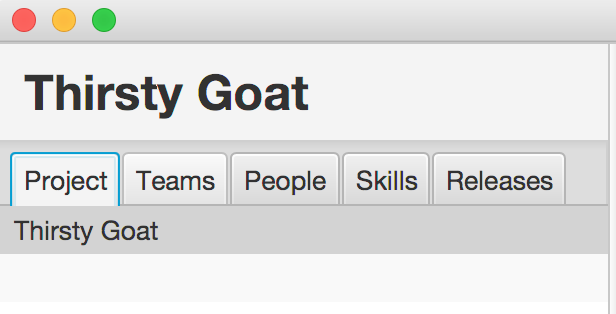
\includegraphics[scale=0.32]{listView}
%  \caption{The list view.\label{listView}}
%\end{figure}
%
%\subsection{Details Pane}
%\begin{itemize}
%  \item Selecting an item from the list (Person, Project, etc) displays the details about that item in the details pane.
%\end{itemize}
%
%\begin{figure}[H]
%  \centering
%  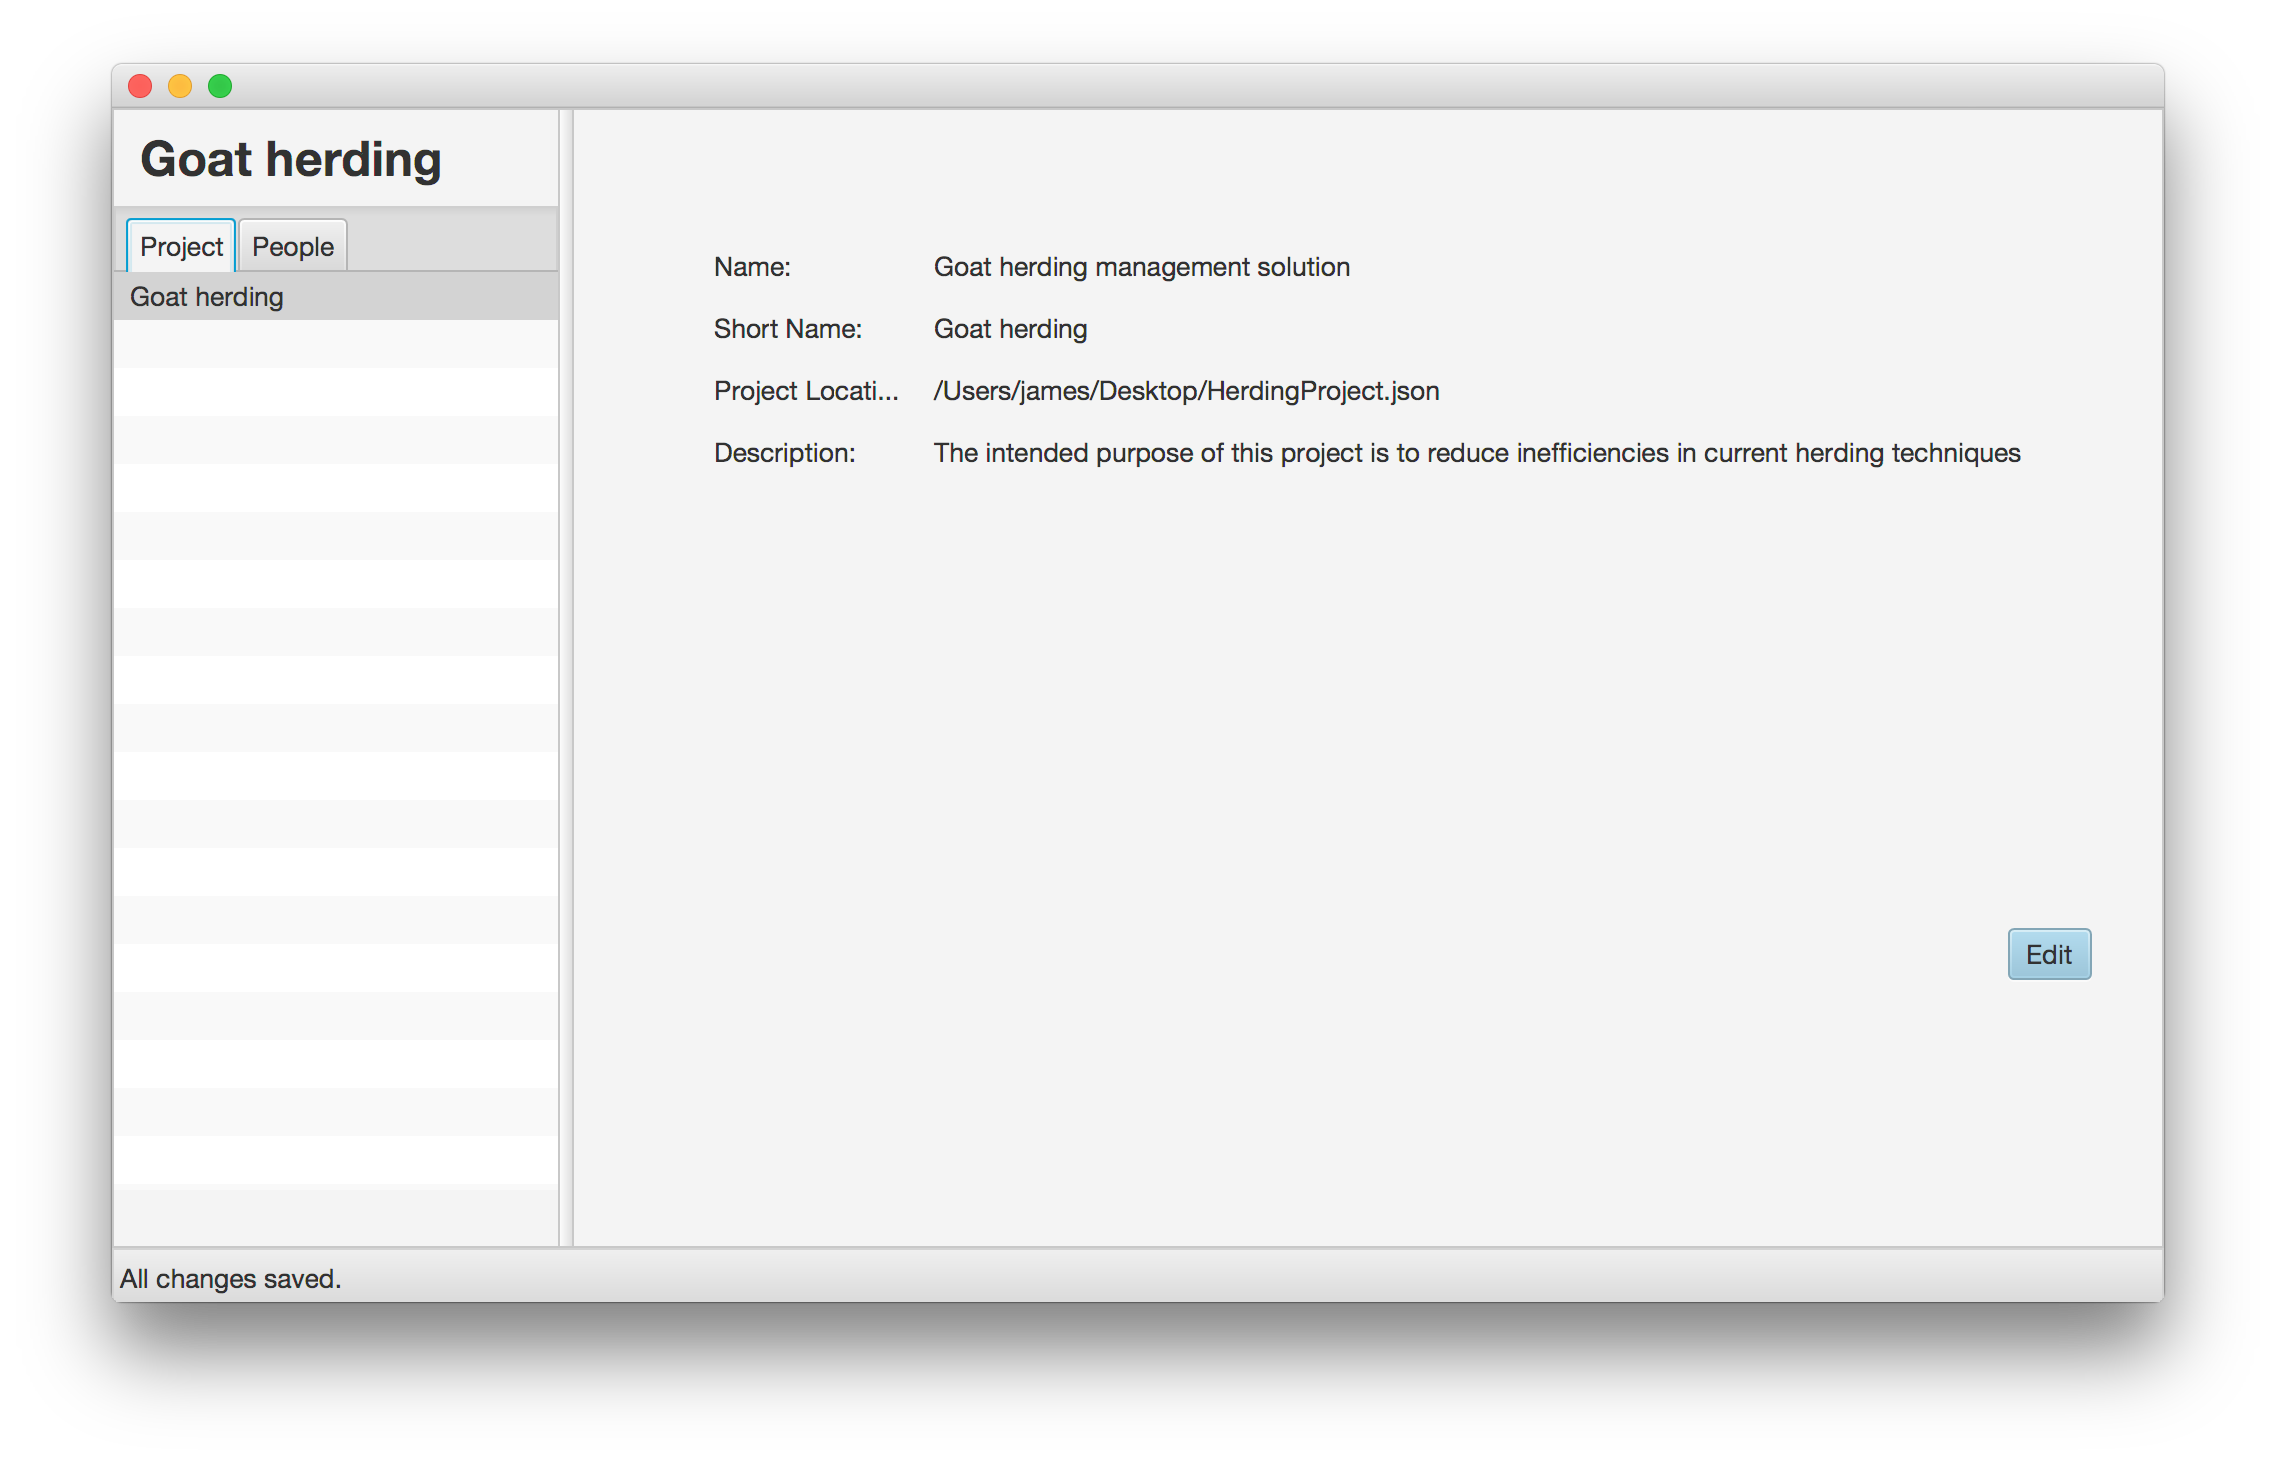
\includegraphics[scale=0.32]{detailsPane}
%  \caption{The details pane.\label{detailsPane}}
%\end{figure}
%
%\subsection{Revert}
%Revert allows a user to discard all unsaved changes and go back to the state where the project was last saved.
%If a project has not been saved then it reverts back to the state when it was last opened.
%\begin{itemize}
%  \item \menu{File > Revert} Prompts the user to Save As before reverting the project's unsaved changes.
%  \item Functionality exists to undo/redo a revert.
%\end{itemize}
%
%\appendix
%\chapter{Appendix}
%
%\subsection{UX Design}
%\begin{itemize}
%\item Click the arrow inside the tree to expand nodes.
%\end{itemize}
%
%\begin{figure}[H]
%  \centering
%  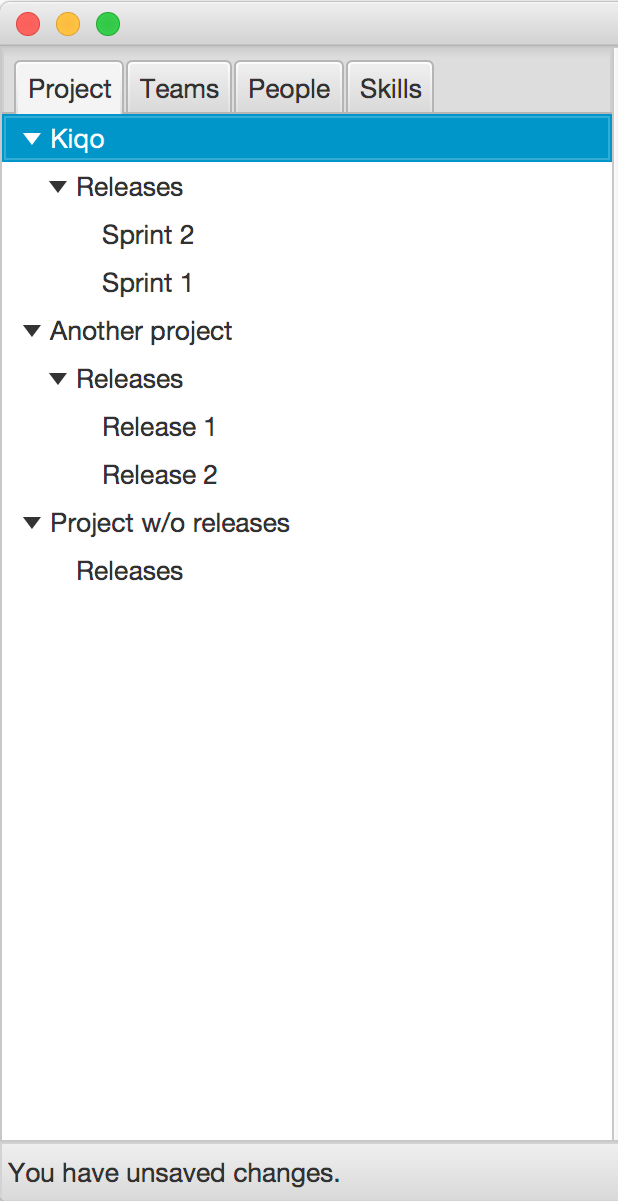
\includegraphics[scale=0.32]{treeView}
%  \caption{The tree view.\label{treeView}}
%\end{figure}
%
%\subsection{Validation}
%User inputs with red triangles in the top left hand corner (See Figure xyz) show that the field is being validated
%
\end{document}
